\chapter[Lezione VII]{Lezione VII\newline\small{\emph{05/05/2011}}}
	\section{Notazioni algebriche}
Si consideri una qualsiasi operazione algebrica. Fino ad ora, si sono adoperate soltanto sintassi in cui l'operatore s'inserisce tra i due operandi (ad esempio, \lstinline!3+4!). Questo tipo di notazione si dice \emph{infissa}. In questa forma, espressioni complicate o lunghe richiedono l'uso di parentesi (come \lstinline!5*(3+4)!).

Si prenda la seguente espressione: \lstinline!5*{[(9+8)*(4+6)]+7}! (notazione infissa); esiste un altro modo di rappresentarla. \`E, infatti, possibile usare la forma \emph{postfissa} (o polacca) e riscriverla in questo modo: \lstinline!5 9 8 + 4 6 + * 7 + *!. La notazione postfissa prevede, come si evince dall'esempio, che l'operatore algebrico segua i due operandi. Nel caso più semplice, \lstinline!3+4! diventa \lstinline!3 4 +!. L'espressione si risolve nel modo usuale:
\begin{center}
\begin{verbatim}
5 9 8 + 4 6 + * 7 + * =
5 17 10 * 7 + * =
5 170 7 + * = 5 177 * = 885
\end{verbatim}
\end{center}


	\section{Strutture Dati}
		\subsection{Stack}
		\label{subsec:stack}
Gli aspetti caratteristici di una struttura dati dati sono:
\begin{itemize}
	\item
I valori che riesce ad assumere (quindi le grandezze che può rappresentare);
	\item
Le operazioni che posso compiere sulla struttura.

\end{itemize}
Per i tipi primitivi, le operazioni definite sono piuttosto implicite e date per scontate fino a questo momento. In ogni caso, si tratta di operazioni algebriche di base (somma, prodotto, resto\dots).
Sfruttando la notazione postfissa, è possibile creare una struttura dati che definisce un particolare procedimento per risolvere un espressione.

Si immagini \marginpar{Operazioni \lstinline!pop! e \lstinline!push!} di avere una \emph{pila} (in inglese, \emph{stack}) di dischetti. Ogni dischetto può memorizzare uno ed un solo numero. Sulla pila è possibile compiere solo due operazioni (vedi la figura~\vref{fig:poppush}):
\begin{itemize}
	\item
\lstinline!push:! mettere un dischetto in cima alla pila;
	\item
\lstinline!pop:! togliere un dischetto dalla cima della pila.
\end{itemize}
Questo procedimento definisce, per i dati, una disciplina del tipo LIFO (\emph{Last In Firs Out}). L'ultimo elemento inserito, cioè, è il primo ad essere prelevato.

Ora, si vuole creare un algoritmo che permetta di risolvere delle espressioni scritte in notazione postfissa sfruttando le operazioni concesse dagli stack. Si potrebbe immaginare di memorizzare nei dischetti numeri immessi (\lstinline!push!) finché non si legge un operatore matematico. A questo punto, si estraggono i due dischetti che si trovano in cima alla pila (\lstinline!pop!) e si esegue su di essi l'operazione richiesta dall'operatore immesso. Successivamente, si memorizza il risultato dell'operazione su un dischetto e lo si mette in cima alla pila (\lstinline!push!).
\begin{wrapfloat}{figure}{i}{0pt}
	\centering
	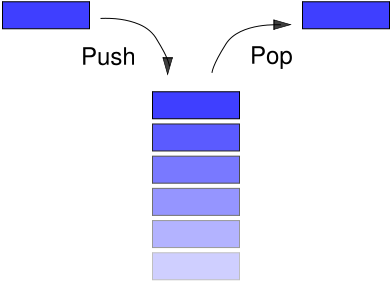
\includegraphics[width=0.4\columnwidth]{immagini/pop_push}
	\caption[Stack]{Rappresentazione delle funzioni \lstinline!pop()! e \lstinline!push()! su uno stack.}
	\label{fig:poppush}
\end{wrapfloat}
\begin{table}
	\centering
	\caption[Stack]{La tabella mostra il contenuto dello stack ad ogni iterazione (tempo).}
	\label{tab:stack}
	\begin{tabular}{ l | l l l l l l l l l l l }
		\toprule
Tempo 			&0	&1 	&2 	&3 	&4 	&5 	&6 	&7 	&8 	&9 	&10	\\
		\midrule
\multirow{4}*{Pila}   	&5 	&9 	&8 	&17 	&4	&6	&10	&170	 &7 	&177	&855  \\
				&	&5	&9	&5	&17	&4	&17	&5	&170	&5	&	\\
				&	&	&5	&	&5	&17	&5	&	&5	&	&	\\
				&	&	&	&	&	&5	&	&	&	&	&	\\
	\end{tabular}
\end{table}
In questo modo\marginpar{Prototipi delle funzioni \lstinline!pop()! e \lstinline!push()!} è possibile calcolare l'espressione precedente. In questo caso, la tabella \ref{tab:stack} mostra i valori presenti nello stack durante l'esecuzione dell'algoritmo.

Si supponga che sia stato definito un tipo di dato \lstinline!stack! in linguaggio C. Si crea, allora, un prototipo della funzione \lstinline!push!: \lstinline!stack push (stack s, int v )!. Si può assumere che la funzione \lstinline!push! riceva come argomento un numero (nella fattispecie, un intero) e lo stack su cui inserirlo, e restituisca uno stack diverso. La funzione \lstinline!pop!, produrrebbe un nuovo stack e un intero. Tuttavia, in C, una funzione può produrre un solo valore. Allora, si ricorre ad un piccolo ""trucchetto'': definendo un solo stack, tutte le funzioni possono solo lavorare su di esso e non c'è più bisogno d'inserirlo né tra gli argomenti della funzione, né nel suo codominio.

Ora, bisogna costruire un tipo di dato che permetta di rappresentare uno stack. Esistono diverse opzioni. Una delle più comode, per il momento, resta costruire un array (vedi anche il paragrafo~\vref{sec:vari:stack}). Esso, tuttavia, è una struttura dati non dinamica: la sua lunghezza non cambia. Si tratterà questo problema più avanti (nel paragrafo~\vref{sec:malloc()}). Per ora, si assuma di aver dichiarato un array di dimensioni sufficienti per contenere tutti i dati inseriti. Si può pensare di riempire il vettore dalla posizione più piccola (\lstinline!0!) e continuare progressivamente verso quella più grande. Per tenete traccia del primo elemento vuoto del vettore, c'è bisogno di dichiarare una variabile ausiliaria (in questo caso di tipo \lstinline!int!). Il codice~\vref{cod:stack} esemplifica quanto detto finora. È importare tenere presente, tuttavia, che la funzione \lstinline!push! dà errore (di \emph{segmentazione}) se \lstinline!valori.indice == N!. Analogamente, la funzione \lstinline!pop! dà errore se il vettore \lstinline!valori.val! è vuoto. Infatti, se \lstinline!valori.indice == 0!, la funzione \lstinline!pop! dà errore (ancora di segmentazione). Vi si può rimediare semplicemente introducendo delle scelte.

\begin{lstlisting}[caption={[{\em Costruzione di uno stack.}]{\em Costruzione di uno stack. In questo esempio s'è usato un record per raggruppare la pila e l'intero che punta al primo elemento vuoto.}}, label={cod:stack}]
/* stack */
struct pila {
	char val[N];
	int indice;
} valori;

void push (char v) {
	valori.val[valori.indice] = v;
	valori.indice++;
}

/* senza argomenti */
char pop (void) {
	valori.indice--;
	return valori.val[valori.indice];
}
\end{lstlisting}

	\section{Allocazione dinamica della memoria}
	\label{sec:malloc()}
Si è già detto che il vettore, come tutte le strutture dati viste finora, è un modello di dati \emph{statico}. Una volta dichiarato, ha una lunghezza fissa. In C, tuttavia, è possibile riservare più spazio ad una o più variabili durante l'esecuzione di un programma.

La\marginpar{La funzione \lstinline!malloc();!} funzione \lstinline!malloc(size_t N);! permette di riservare \lstinline!N byte!  per l'assegnamento di una variabile. Anche se non è stata ancora introdotta la locuzione \lstinline!size_t N!, si vede chiaramente che si riferisce al numero di \lstinline!byte!\footnote{Un \lstinline!byte! può contenere un carattere. Generalmente, un intero occupa \lstinline!4 byte!. Questo, tuttavia, non è sempre vero.} che si chiede di riservare. Inoltre, \lstinline!N! è sempre (strettamente) maggiore di zero. La funzione \lstinline!malloc(size_t N);!, in realtà, restituisce un puntatore di tipo speciale \lstinline!void! (\lstinline!void * malloc(size_t N);!). Questo crea un'inconsistenza formale, poiché tale tipo non corrisponde a quello del puntatore che si è dichiarato. Anche se il calcolatore tollera tale inconsistenza, è sempre meglio operare un \lstinline!cast!, come nel codice~\vref{cod:malloc()}, specificando tra parentesi il tipo di puntatore davanti alla funzione \lstinline!malloc(...);!: \lstinline! n = (tipo *)malloc(sizeof(tipo));!. La funzione \lstinline!sizeof(tipo);! (alle righe 9 e 14) restituisce il numero di \lstinline!byte! occupato dal tipo di dato specificato come argomento.

La\marginpar{\lstinline!malloc();! e gli array} funzione \lstinline!malloc();! assume una forma particolarmente comoda per la dichiarazione e l'uso di array. Nel codice~\vref{cod:malloc()} (riga 14), ad esempio, si chiede riservare lo spazio per \lstinline!100! interi. Esso sarà contiguo e quindi adatto ad essere indicizzato tramite un vettore. La stretta relazione tra il nome di un array e i puntatori cui si è accennato in precedenza permette di effettuare degli assegnamenti come quelli nell'ultima riga.
\begin{lstlisting}[caption={[\em Uso della funzione \lstinline!malloc();!.]{\em Uso della funzione \lstinline!malloc();!. Si  faccia particolare attenzione a non dimenticare d'inserire la scelta immediatamente dopo aver richiamato tale funzione.}}, label={cod:malloc()}]
struct nodo {
	int val;
	char c;
} x, *p, *n;
int *pn;
...
p = &x; /* assegno a p l'indirizzo di x */
(*p).val = 0; /* assegno 0 a x.val */
n = (struct nodo *)malloc(sizeof(struct nodo));
if ( n == NULL )
	exit(EXIT_FAILURE);
(*n).val = 10;

pn = (int *)malloc(100*sizeof(int));
if ( pn == NULL )
	exit(EXIT_FAILURE);
pn[10] = 1;
\end{lstlisting}

Bisogna prestare particolare attenzione al fatto che, qualora la funzione \lstinline!malloc(...);! non trovi abbastanza spazio contiguo da allocare, ritorna con il valore \lstinline!NULL!, \marginpar{Valore NULL} valido come puntatore, ma non come indirizzo. Allora, si fa seguire ad ogni istruzione \lstinline!malloc(...);! la scelta\footnote{Il professor Bernardinello ha tenuto a specificare che la mancata introduzione della scelta dopo tale funzione verrà considerata errore.} mostrata nel codice~\vref{cod:malloc()}.

	\section{Strutture dati}
		\subsection{Liste Concatenate}
		\label{subsec:liste}
%\begin{wrapfloat}
\begin{figure}
%{i}{0pt}
	\centering
	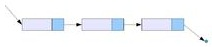
\includegraphics[width=0.4\columnwidth]{immagini/lista}
	\caption[Lista concatenata monodirezionale]{Lista concatenata monodirezionale. I campi in blu sono puntatori.}
	\label{fig:mlist}
\end{figure}
%{wrapfloat}
Con questi strumenti è possibile costruire qualcosa che somigli più di un array ad uno stack. L'idea è di comporre una \emph{lista concatenata}, ossia una sequenza di strutture (record) con gli stessi campi che dal punto di vista logico sono ordinate tramite un dato criterio. Esse sono generalmente ""collegate'' da puntatori (vedi la figura~\ref{fig:mlist}). Le strutture che compongono una lista, infatti, non occupano posizioni contigue in memoria ma, nella maggior parte dei casi, sono ""sparpagliate''. Qui intervengono i puntatori: ogni struttura dovrà contenere un campo che punti all'elemento successivo della lista. L'ultimo elemento avrà il campo puntatore contenente il valore \lstinline!NULL! (per segnare la fine della lista). Questi accorgimenti consentono d'inserire altri record in qualsiasi posizione della lista.

Si può ora rappresentare uno stack tramite una lista concatenata. Ovviamente, servirà un puntatore ""esterno'' (chiamato generalmente \lstinline!*testa!) che punti al nodo che si trova ""in alto'' nella pila, analogamente a quanto si è fatto con gli array.
\begin{lstlisting}
struct nodo {
	int v;
	char c;
	struct nodo *next;
}
\end{lstlisting}